\newcommand{\shelltext}[1]{
  \textsf{\tiny{#1}}
}

\newcommand{\commitnode}[7]{
  {
    \path[color=#7]<#6> node[#1, fill=white!#2, minimum width= 2.4cm, minimum height=1.2cm, text width=2.2cm, align=left] (cnew)
    (#5) at #3  [draw] {\vbox to 1cm{\vfill \hbox{\shelltext{#4}}}};
  }
}


\newcommand{\commitgroup}[5]{
  \begin{scope}[shift={#1}, scale=#2,
    every node/.append style={transform shape} % from https://tex.stackexchange.com/a/350127
    ]
    \commitnode{}{100}{(0.3,-0.7)}{...........}{others_#3}{#4}{#5}
    \commitnode{}{100}{(0.2,-0.4)}{54a78ac2...}{c1_#3}{#4}{#5}
    \commitnode{}{100}{(0.1,-0.1)}{deadbeef...}{c2_#3}{#4}{#5}
    \commitnode{}{100}{(0.0, 0.2)}{eaf329aa...}{c3_#3}{#4}{#5}
    \commitnode{dotted}{100}{(-0.1,0.5)}{\tiny{$<$new commit$>$}}{cnew_#3}{#4}{#5};
  \end{scope}
}

\definecolor{addcolor}{rgb}{0.0,0.5,0.0}
\definecolor{commitcolor}{rgb}{0.6,0.0,0.0}
\definecolor{commit-a-color}{rgb}{0.6,0.3,0.3}
\definecolor{restorecolor}{rgb}{0.0,0.0,0.7}
\definecolor{resetcolor}{rgb}{0.3,0.3,0.3}
\definecolor{remotecolor}{rgb}{0.45,0.45,0.45}
\definecolor{cloudremotecolor}{rgb}{0.65,0.65,0.65}
\definecolor{cloudremotecolor2}{rgb}{0.75,0.75,0.75}


\begin{frame}{The 3 Kinds of State of a File in Git}
  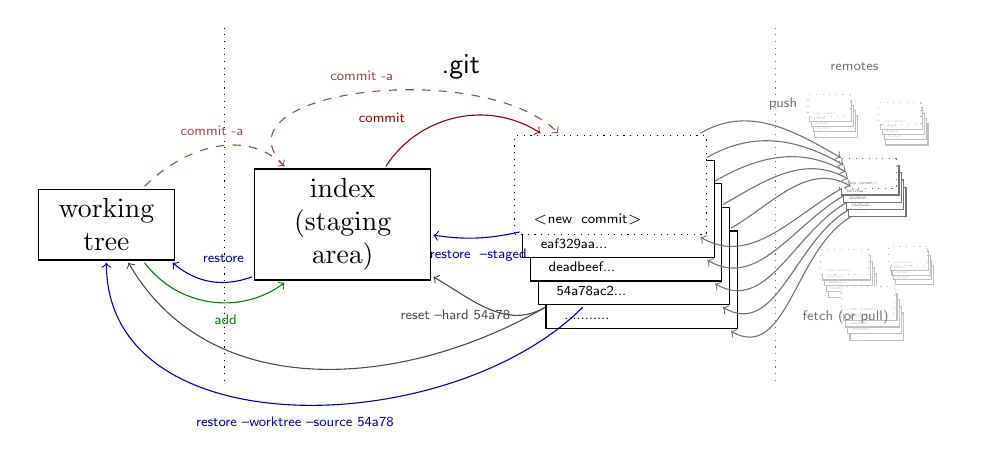
\begin{tikzpicture}[outer sep=1]
    \path [use as bounding box] (-1.0,-0.5) rectangle (11,4.5);


    % this is the only version of your file that applications outside of git see.
    \path[]<1-> node[text width=1.5cm, align=center](wt)   at (0,2)  [draw] {working tree};
    \path[draw]<1-> [dotted] (1.5,4.5) -- (1.5,0);

    % when git comes into play, many more versions become available
    \path[]<2-> node[text width=1.5cm, align=center] (git)   at (4.5,4)  {\textsf{.git}};

    % there is the staging area
    \path[]<2->  node[text width=2.0cm, align=center] (idx)   at (3,2)  [draw] {index \\ (staging area)};


    \commitgroup{(6.5,2.0)}{1.0}{local}{2-}{black}

    % git add copies the version of a file to the index
    % that it, it overwrites the version in the index.

    \path[draw,->,color=addcolor]<3-> (wt) edge [ bend right=45] node[pos=0.60, below] {\shelltext{add}} (idx) ;

    % new commit


    \path[draw,->, auto=left, color=commitcolor]<4-> (idx) edge [ bend left=45 ]
    node[pos=0.25] {\shelltext{commit}} (cnew_local) ;


    % there are also remotes!

    \path[draw,dotted,color=remotecolor]<2-> (8.5,4.5) -- (8.5,0);
    \path[color=remotecolor]<2-> node[text width=1.5cm, align=center] (origin)   at (9.5,4)  {\shelltext{remotes}};

    \commitgroup{(9.7,2.5)}{0.3}{remote}{2-}{remotecolor}

    \commitgroup{(10.1,3.3)}{0.22}{remote_7}{2-5}{cloudremotecolor}
    \commitgroup{(9.2,3.4)}{0.22}{remote_7}{2-5}{cloudremotecolor}
    \commitgroup{(10.2,1.5)}{0.2}{remote_2}{2-5}{cloudremotecolor}
    \commitgroup{(9.4,1.4)}{0.25}{remote_4}{2-5}{cloudremotecolor}
    \commitgroup{(9.7,0.9)}{0.28}{remote_5}{2-5}{cloudremotecolor}



    % one can also commit directly from the worktree

    \path[draw,->, auto=left, color=commit-a-color]<3-> (idx) edge [ out=135,in=135, dashed ]
    node[pos=0.5, color=commit-a-color, above] {\shelltext{commit -a }}
    (cnew_local) ;

    % this affects also the index
    \path[draw,->, color=commit-a-color]<3-> (wt) edge [ out=45, in=135, dashed ]
    node[pos=0.5, color=commit-a-color, above] {\shelltext{commit -a }}
    (idx) ;

    % there's also restore in its different incarnations
    \path[draw,->, color=restorecolor]<4-> (c3_local) edge [bend left = 10 ]
    node[pos=0.3, text width=1.6cm, below ] {\shelltext{restore --staged }} (idx);
    \path[draw,->, color=restorecolor]<4-> (c1_local) edge [out=225,in=270] node[pos=0.5,below] {\shelltext{restore --worktree --source 54a78}} (wt);
    \path[draw,->, auto=right, color=restorecolor]<5-> (idx) edge [bend left = 30 ] node[pos=0.75] {\shelltext{restore}} (wt);

    % and reset, although reset is primarily an operation on HEAD
    \path[draw,->,color=resetcolor]<5-> (c1_local) edge [out=210, in=330] node[pos=0.20, left] {\shelltext{reset --hard 54a78}} (idx);
    \path[draw,->,color=resetcolor]<5-> (c1_local) edge [out=210, in=300] (wt);


    % new commits are pushed to a remote with push
    \commitgroup{(10.1,3.3)}{0.22}{remote_7}{6-}{cloudremotecolor2}
    \commitgroup{(9.2,3.4)}{0.22}{remote_7}{6-}{cloudremotecolor2}
    \commitgroup{(10.2,1.5)}{0.2}{remote_2}{6-}{cloudremotecolor2}
    \commitgroup{(9.4,1.4)}{0.25}{remote_4}{6-}{cloudremotecolor2}
    \commitgroup{(9.7,0.9)}{0.28}{remote_5}{6-}{cloudremotecolor2}



    \path[draw,->,color=remotecolor]<6-> (others_local) edge [out=30, in=150]  (others_remote);
    \path[draw,->,color=remotecolor]<6-> (c1_local) edge [out=30, in=150]  (c1_remote);
    \path[draw,->,color=remotecolor]<6-> (c2_local) edge [out=30, in=150]  (c2_remote);
    \path[draw,->,color=remotecolor]<6-> (c3_local) edge [out=30, in=150]  (c3_remote);
    \path[draw,->, auto=left,color=remotecolor]<6-> (cnew_local) edge [out=30, in=150] node [pos=0.4] {\shelltext{push}} (cnew_remote);

    % and they are fetched by fetch or pull
    \path[draw,->, auto=left,color=remotecolor]<6-> (others_remote) edge [in=330, out=210] node [pos=0.5] {\shelltext{fetch (or pull)}}  (others_local);
    \path[draw,->,color=remotecolor]<6-> (c1_remote) edge [in=330, out=210]  (c1_local);
    \path[draw,->,color=remotecolor]<6-> (c2_remote) edge [in=330, out=210]  (c2_local);
    \path[draw,->,color=remotecolor]<6-> (c3_remote) edge [in=330, out=210]  (c3_local);
    \path[draw,->,color=remotecolor]<6-> (cnew_remote) edge [in=330, out=210]  (cnew_local);



  \end{tikzpicture}

  \begin{minipage}[b][3cm][b]{1.0\textwidth}
  \only<1> {
    The plain directory.\\
    Every other application than Git sees only this.}
  \only<2> {
    With Git, we have different versions to each tracked file of your project:
    \begin{itemize}
      \item The version in the working tree
      \item The version in the INDEX (also referred to as ``staging area'')
      \item A version for each commit
    \end{itemize}


    \textbf{How can we copy the state of a file between versions?}
  }

  \only<3>{The most used git commands:
    \textsf{\textcolor{addcolor}{add}}
    and \textsf{\textcolor{commitcolor}{commit}}}

  \only<4>{Take the version of a file from a commit: \textsf{\textcolor{restorecolor}{restore}}}
  \only<5>{Take the version of a file from a commit: \textsf{\textcolor{resetcolor}{reset}}.
    Reset (primarily) moves HEAD
  }

  \only<6>{
    Notes: push, fetch and pull work on commits (and referenced objects),
    not on single files!
  }
  \only<7>{}
  \end{minipage}
\end{frame}
